\subsection{Kiểm định hai mẫu: Nvidia vs AMD}

\subsubsection{Mục tiêu phân tích}
Sau khi thấy hiệu năng chung chưa đạt mục tiêu, nhóm thực hiện so sánh trực tiếp biến \texttt{Pixel\_Rate} giữa hai đối thủ chính là Nvidia và AMD. Việc này giúp nhóm xác định xem có sự phân hóa đáng kể về năng lực công nghệ giữa hai nhà sản xuất này hay không.

\subsubsection{Thiết lập giả thuyết kiểm định}
\begin{itemize}
    \item \textbf{Giả thuyết không ($H_0$):} $\mu_{Nvidia} = \mu_{AMD}$ (Không có sự khác biệt về hiệu năng giữa hai hãng).
    \item \textbf{Đối thuyết ($H_1$):} $\mu_{Nvidia} \neq \mu_{AMD}$ (Có sự khác biệt đáng kể giữa hai hãng).
\end{itemize}

\subsubsection{Quy trình các bước thực hiện và phân tích kịch bản}
Nhóm xây dựng kịch bản lựa chọn phép thử:
\begin{enumerate}
    \item \textbf{Kịch bản 1: Cả hai nhóm đạt tính chuẩn.} Nhóm sẽ dùng T-test (Student nếu phương sai bằng nhau, Welch nếu phương sai khác nhau).
    \item \textbf{Kịch bản 2: Vi phạm tính chuẩn.} Nhóm sẽ sử dụng \textbf{Mann-Whitney U Test}. Đây là lựa chọn tối ưu để so sánh vị trí trung tâm dựa trên thứ hạng thay vì trung bình cộng, giúp kết quả ổn định hơn trước các biến động dữ liệu.
\end{enumerate}

\subsubsection{Triển khai tuần tự các bước bằng code R}
\textbf{Bước 1: Kiểm tra tính chuẩn theo từng nhóm}
\begin{lstlisting}
df_compare %>% group_by(Manufacturer) %>% summarise(p_val = shapiro.test(Pixel_Rate)$p.value)
\end{lstlisting}

\textbf{Kết quả:}
\begin{figure}[H]
    \centering
    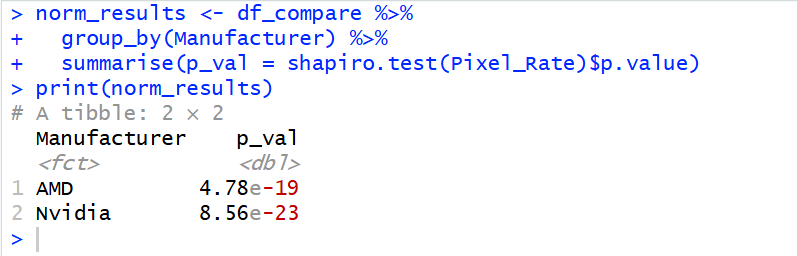
\includegraphics[width=1\linewidth]{../images/7.1.png}
    \caption{Kiểm tra tính chuẩn theo nhà sản xuất}
\end{figure}

\textbf{Đánh giá:} Cả hai hãng đều có $p < 0.05$. Nhóm xác định đi theo hướng kiểm định phi tham số.

\textbf{Bước 2: Kiểm tra đồng nhất phương sai}
\begin{lstlisting}
car::leveneTest(Pixel_Rate ~ Manufacturer, data = df_compare)
\end{lstlisting}

\textbf{Kết quả:}
\begin{figure}[H]
    \centering
    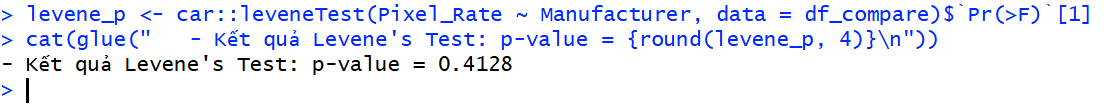
\includegraphics[width=1\linewidth]{../images/7.2.png}
    \caption{Kết quả kiểm định Levene cho phương sai}
\end{figure}


\textbf{Đánh giá:} $p\text{-value} = 0.4128 > 0.05$, phương sai đồng nhất. Tuy nhiên do vi phạm tính chuẩn ở bước 1, nhóm chính thức sử dụng Mann-Whitney U.

\textbf{Bước 3: Thực hiện kiểm định chính và tính Cohen's d}
\begin{lstlisting}
res_two <- wilcox.test(Pixel_Rate ~ Manufacturer, data = df_compare, conf.int = TRUE)
effectsize::cohens_d(Pixel_Rate ~ Manufacturer, data = df_compare)
\end{lstlisting}
\begin{figure}[H]
    \centering
    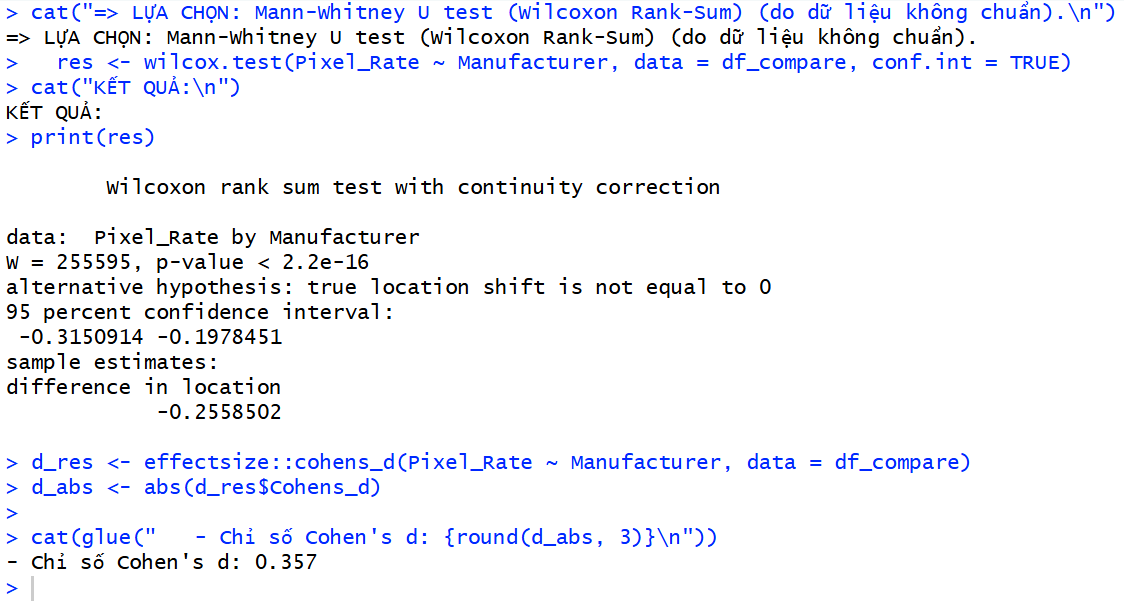
\includegraphics[width=1\linewidth]{../images/7.3.png}
    \caption{Kết quả kiểm định Mann-Whitney U giữa Nvidia và AMD}
\end{figure}

\subsubsection{Phân tích trực quan và kết luận ý nghĩa}
 Nhóm vẽ biểu đồ Violin kết hợp Boxplot nhằm quan sát không chỉ sự khác biệt về trung vị mà còn về mật độ tập trung dữ liệu và mức độ chồng lấn (overlap) giữa hai phân phối, từ đó lý giải cho quy mô thực tế của sự khác biệt.

\begin{figure}[H]
    \centering
    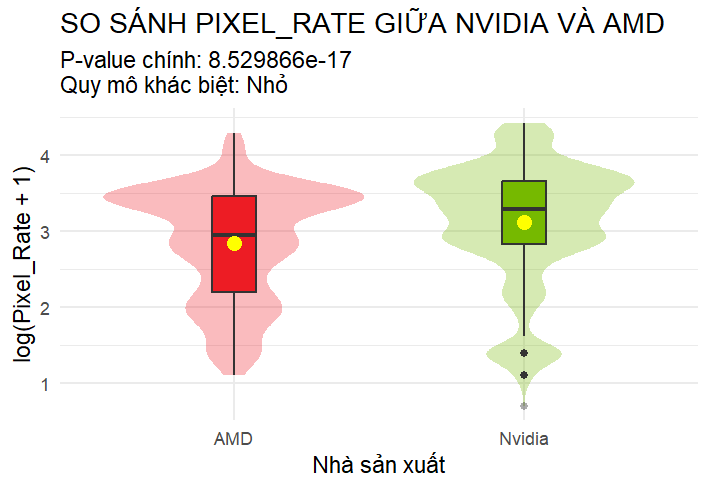
\includegraphics[width=1\linewidth]{../images/7.4.png}
    \caption{So sánh Pixel\_Rate giữa Nvidia và AMD qua biểu đồ Violin}
    \label{fig:violin_2sample}
\end{figure}

\textbf{Phân tích chi tiết biểu đồ và kết luận:}
\begin{itemize}
    \item \textbf{Về hình ảnh:} Điểm vàng (trung bình) của Nvidia nằm cao hơn AMD, tương ứng với giá trị $p < 2.2 \times 10^{-16}$ khẳng định ưu thế của Nvidia có ý nghĩa thống kê. Tuy nhiên, thân của hai khối Violin có phần diện tích chồng lấn rất lớn, cho thấy nhiều dòng GPU của hai hãng vẫn có hiệu năng tương đương nhau.
    \item \textbf{Về ý nghĩa thực tế:} Chỉ số \textbf{Cohen's d = 0.357} (mức độ \textbf{Nhỏ}) phản ánh rằng dù có sự khác biệt rõ rệt về mặt số liệu, nhưng khoảng cách hiệu năng thực tế giữa hai hãng là không quá áp đảo. Kết quả này dẫn dắt nhóm đến bước tiếp theo tại Chương 7: xây dựng mô hình hồi quy đa biến để tìm hiểu các nhân tố kỹ thuật khác ngoài thương hiệu chi phối năng lực GPU.
\end{itemize}
